% ====================================================================
%  RQ3 -- Evaluation under censoring (Chapter 5, ~11 min)
%  Slides 1-5 adapted from the ICML 2026 position paper deck.
%  Layout convention: text/maths left, figure right.
% ====================================================================

\roadmapframe{3}{RQ3. How should survival predictions be evaluated when outcomes are censored, and how can evaluation bias be reduced under dependent censoring?}

% ------------------------------------------------------------- Position paper
% Frames taken verbatim from the ICML 2026 position-paper deck
% (figures in figures/icml/; citations numbered).
\begin{frame}{Diagnosis: evaluation often does not match the goal}\begin{columns}[T]
  \begin{column}{0.54\textwidth}
    \centering
    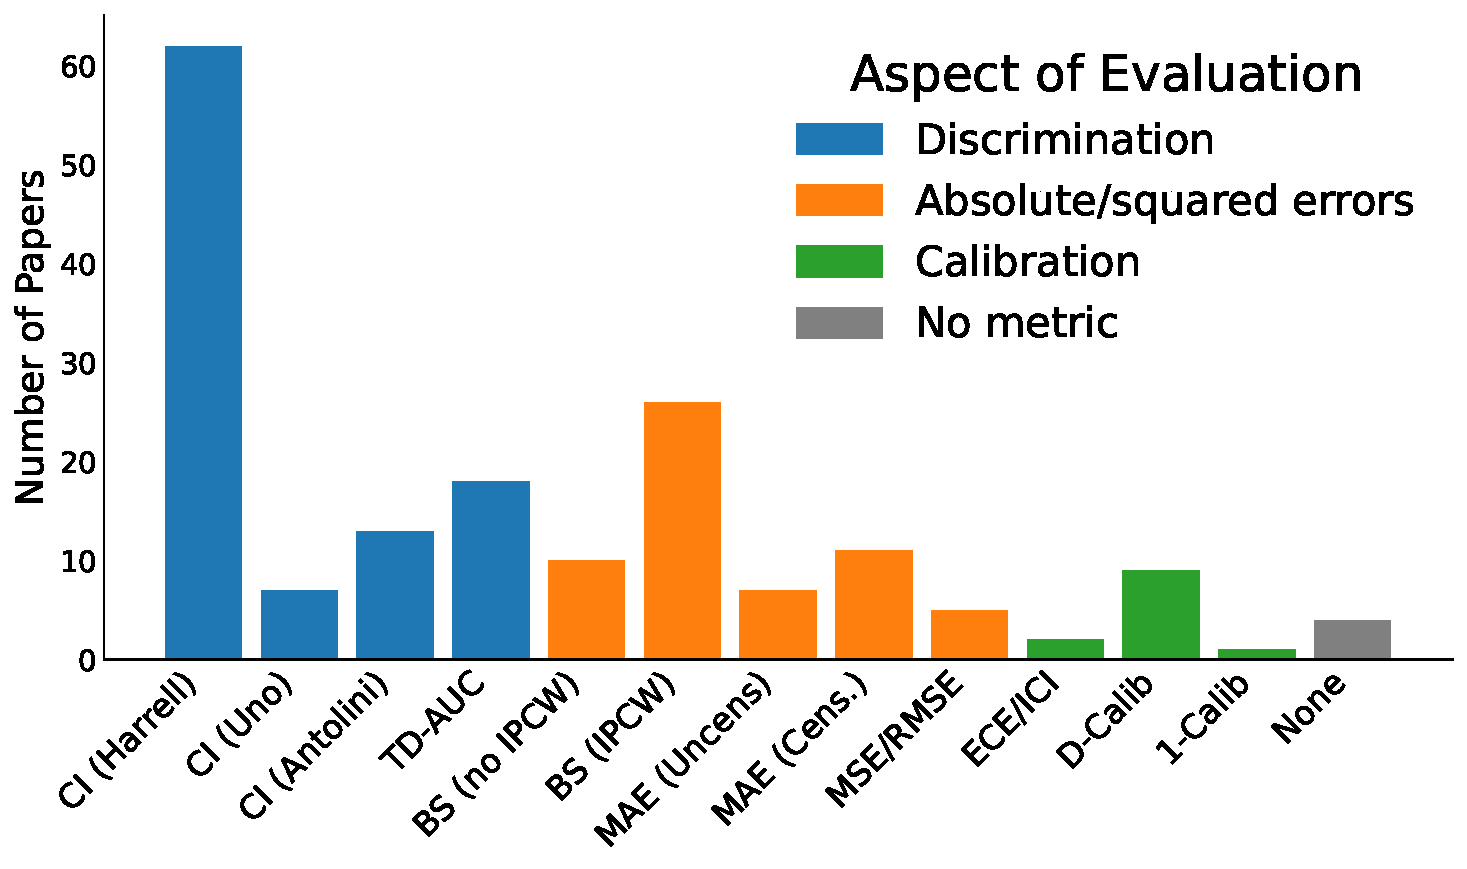
\includegraphics[width=\linewidth]{icml/metrics_used.pdf}
  \end{column}
  \begin{column}{0.35\textwidth}
    \centering
    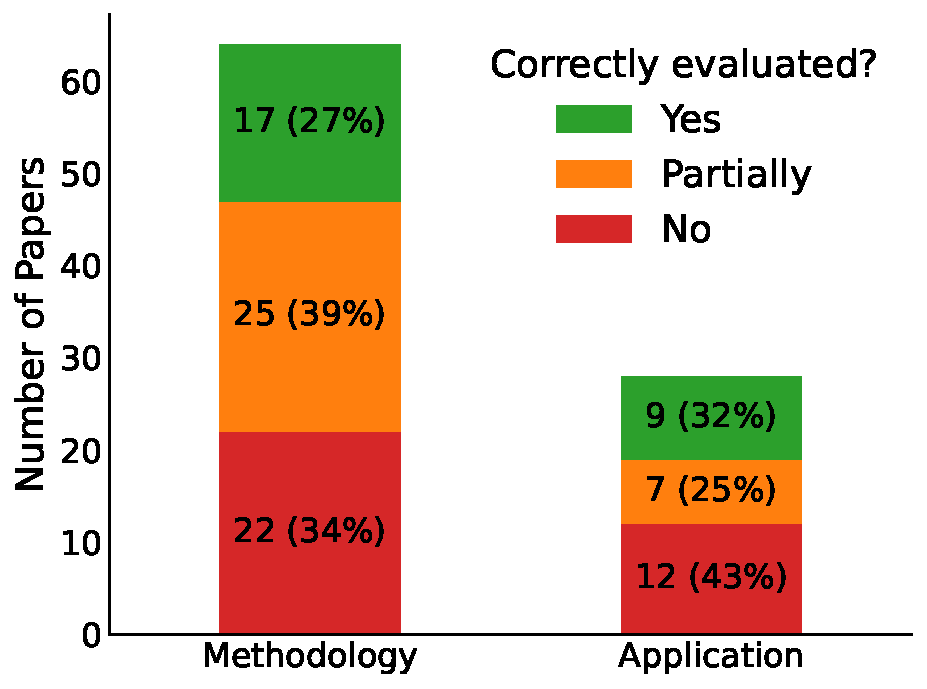
\includegraphics[width=\linewidth]{icml/metrics_correctness.pdf}
  \end{column}
\end{columns}

\vspace{0.6em}
\small
\textbf{Main diagnosis.} Recent survival papers often use discrimination metrics -- especially the C-index -- as a default~\cite{zhou2023survmetrics}, even when the stated goal is time-to-event accuracy or calibrated survival probabilities.

\vspace{0.4em}
\begin{itemize}
  \item The metric answers a different question than the model is designed to solve.
  \item Censoring assumptions are often left implicit, unjustified, or not corrected for.
  \item The result is not just noisy evaluation; it can change the meaning of the claim.
\end{itemize}
\end{frame}

\begin{frame}{The Ladder Hypothesis}\begin{columns}[T]
  \begin{column}{0.50\textwidth}
    \centering
    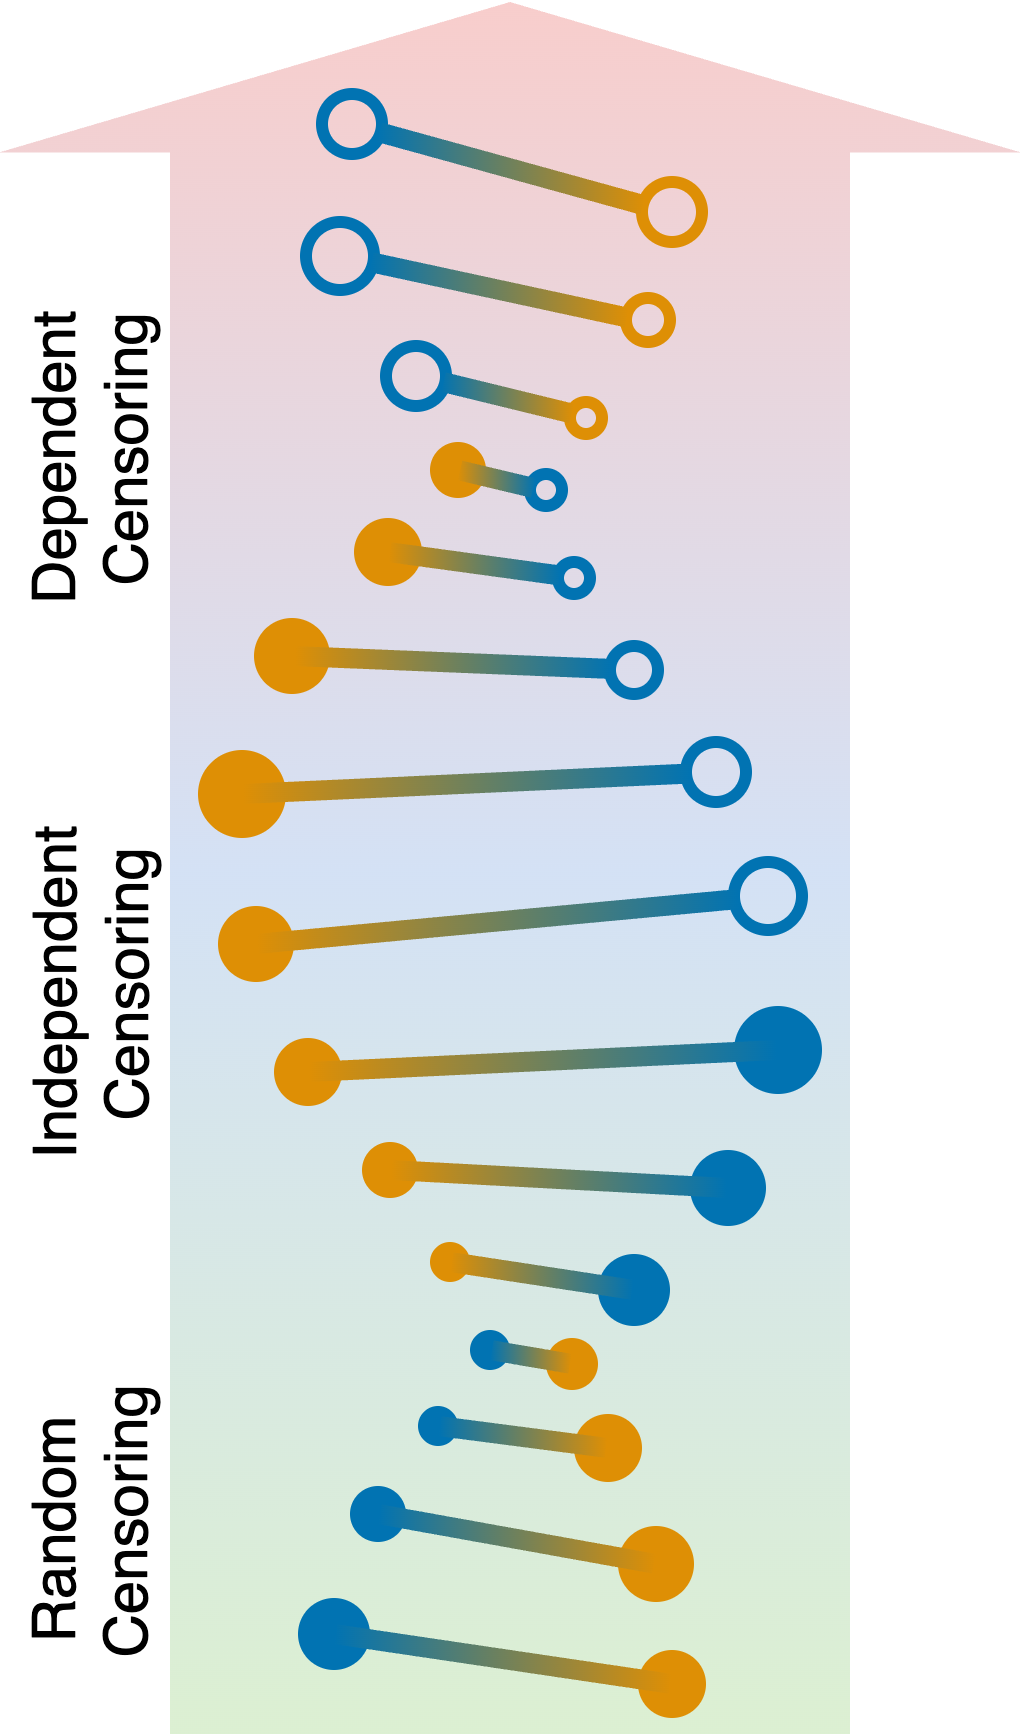
\includegraphics[height=0.65\textheight]{icml/model_vs_evaluation_old.png}
  \end{column}
  \begin{column}{0.50\textwidth}
    \small
    \textbf{Hypothesis.} A model is trustworthy only when it is evaluated using metrics whose validity rests on the same, or weaker, statistical assumptions.

    \vspace{0.6em}
    \begin{itemize}
      \item Models increasingly target weaker assumptions, including dependent censoring.
      \item Standard metrics often still rely on random or independent censoring corrections.
      \item This creates a systematic \emph{model--metric mismatch}.
    \end{itemize}

    \vspace{0.4em}
    \textbf{Consequence:} a better model can look worse, or a biased metric can make an unsupported state-of-the-art claim look convincing.
  \end{column}
\end{columns}
\end{frame}

\begin{frame}{Bias appears when assumptions break}\centering

\begin{minipage}{0.48\linewidth}
    \centering
    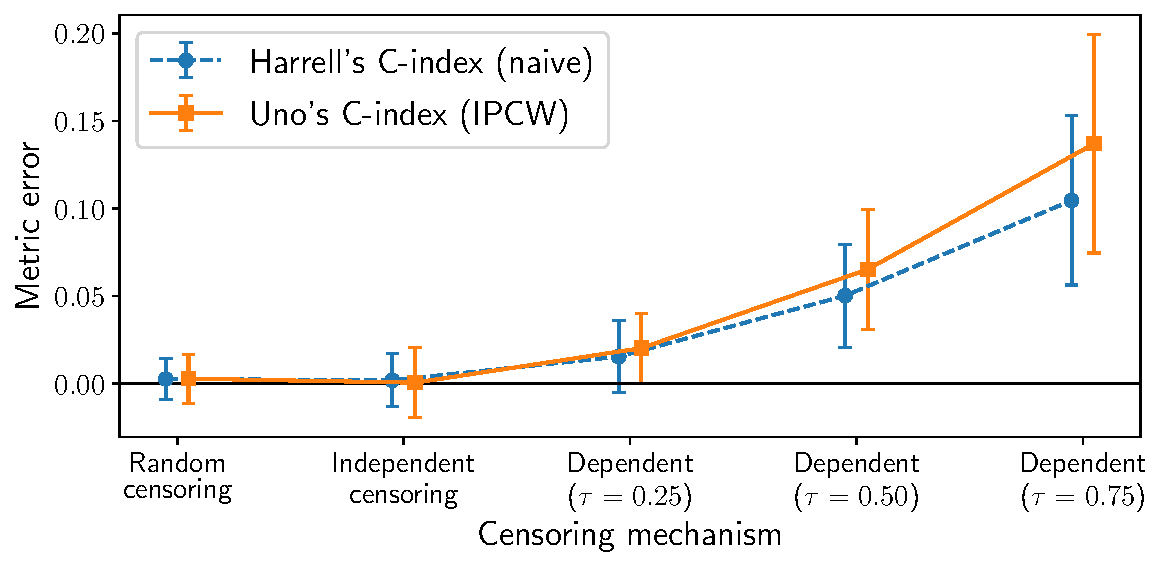
\includegraphics[width=\linewidth]{icml/ci_error_curve.pdf}
    
    \vspace{0.2em}
    {\small CI error under censoring.}
\end{minipage}
\hfill
\begin{minipage}{0.48\linewidth}
    \centering
    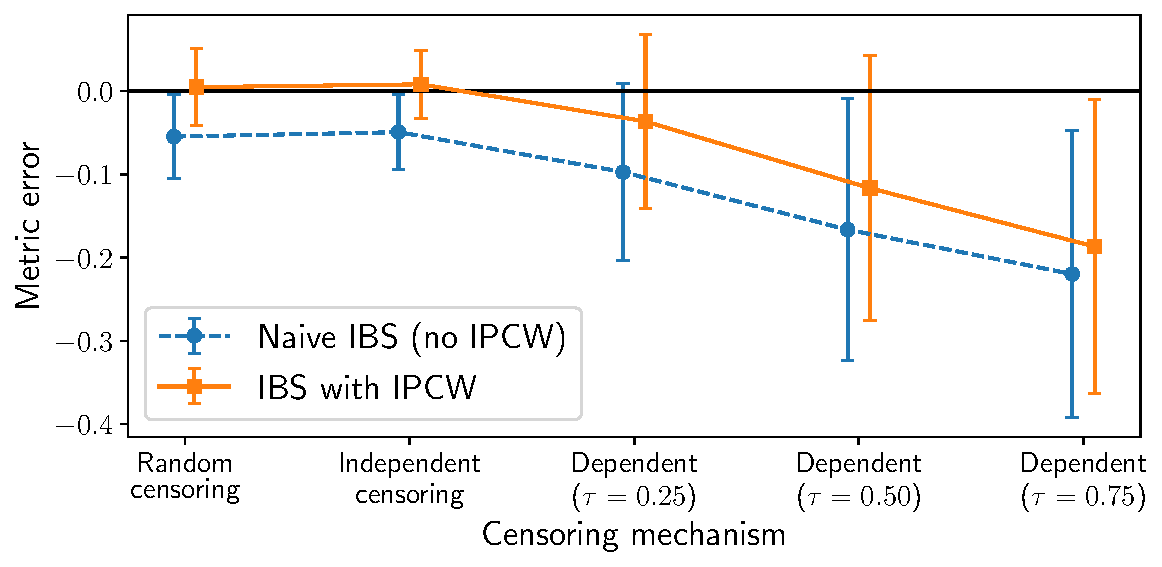
\includegraphics[width=\linewidth]{icml/ibs_error_curve.pdf}
    
    \vspace{0.2em}
    {\small IBS error under censoring.}
\end{minipage}

\vspace{0.4em}
\small
\begin{itemize}
  \item We hold the predictive model fixed and vary only the censoring mechanism.
  \item Errors are computed relative to oracle performance using true event times.
  \item As censoring becomes more dependent, standard CI and IBS estimates drift away from the oracle.
\end{itemize}

\takeaway{The issue is not just which model is better; it is whether the evaluation procedure remains valid under the data-generating assumptions.}
\end{frame}

\begin{frame}{Practical recommendations and alternative views}\small
\begin{columns}[T]
  \begin{column}{0.52\textwidth}
    \textbf{Recommendations}
    \begin{enumerate}
      \item \textbf{Stick to your goal.} Choose the primary metric from the scientific objective: ranking, time-to-event accuracy, calibration, or another target.
      \item \textbf{Evaluate from multiple angles.} For general-purpose methods, report representative discrimination, error-based, and calibration metrics.
      \item \textbf{Strive for consistency.} State the censoring assumption and choose metrics whose correction procedure supports it.
    \end{enumerate}
  \end{column}

  \begin{column}{0.48\textwidth}
    \textbf{Alternative views}
    \begin{itemize}
      \item The C-index is convenient, familiar, and application-agnostic.
      \item Standard metrics preserve comparability with prior work.
      \item If all models are evaluated on the same dataset, the bias may seem shared.
    \end{itemize}

    \vspace{0.4em}
    \textbf{Response.} Convenience does not make a metric assumption-free. Shared biased evaluation can still produce misleading rankings, especially when models make different censoring assumptions.
  \end{column}
\end{columns}
\end{frame}

% ------------------------------------------------------------- Copula Brier
\begin{frame}{Motivation: when dropout depends on what we do not see}
\begin{columns}[c]
  \begin{column}{0.54\textwidth}
    \small
    \textbf{Now: dependent censoring} -- censoring that is related to the event, even given the covariates.
    \vspace{0.5em}

    Cancer patients: $E$ = relapse, $C$ = dropout from the study.
    \vspace{0.4em}
    \begin{itemize}
      \item Patients with a high \textbf{tumor grade} relapse earlier \dots
      \item \dots\ and are also more likely to drop out (too sick to attend).
      \item Tumor grade is \emph{not} recorded in the data.
    \end{itemize}
    \vspace{0.4em}
    $\Rightarrow$ $E$ and $C$ stay dependent, even given the observed $X$:
    \[ E \not\perp C \mid X \]
    \vspace{-0.6em}

    KM and IPCW assume the opposite -- so evaluation becomes biased.
  \end{column}
  \begin{column}{0.44\textwidth}
    \centering
    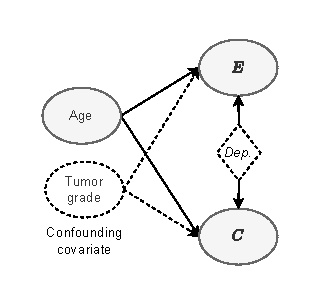
\includegraphics[width=\linewidth]{dependent_censoring.pdf}
    \figsource{Figure from Lillelund et al.~\cite{lillelund_overcoming_2026}}
  \end{column}
\end{columns}
\end{frame}

\begin{frame}{Modelling dependent $E$ and $C$ with a copula}
\begin{columns}[c]
  \begin{column}{0.52\textwidth}
    \small
    A \textbf{copula} glues the two survival functions into a joint one \cite{Sklar1959}:
    \[
      \Pr(E > e, C > c) = \mathcal{C}_\theta\big(S_E(e), S_C(c)\big)
    \]
    \vspace{-0.6em}
    \begin{itemize}
      \item Captures non-linear dependence, e.g.\ strongest in the tails
      \item One parameter $\theta$ sets the strength
    \end{itemize}
    \textbf{Clayton} \cite{clayton1978model}:
    \[
      \mathcal{C}_\theta(u, v) = \big(u^{-\theta} + v^{-\theta} - 1\big)^{-1/\theta}
    \]
    Kendall's $\tau = \frac{\theta}{\theta + 2}$; \;$\tau = 0$: independence.
  \end{column}
  \begin{column}{0.46\textwidth}
    \centering
    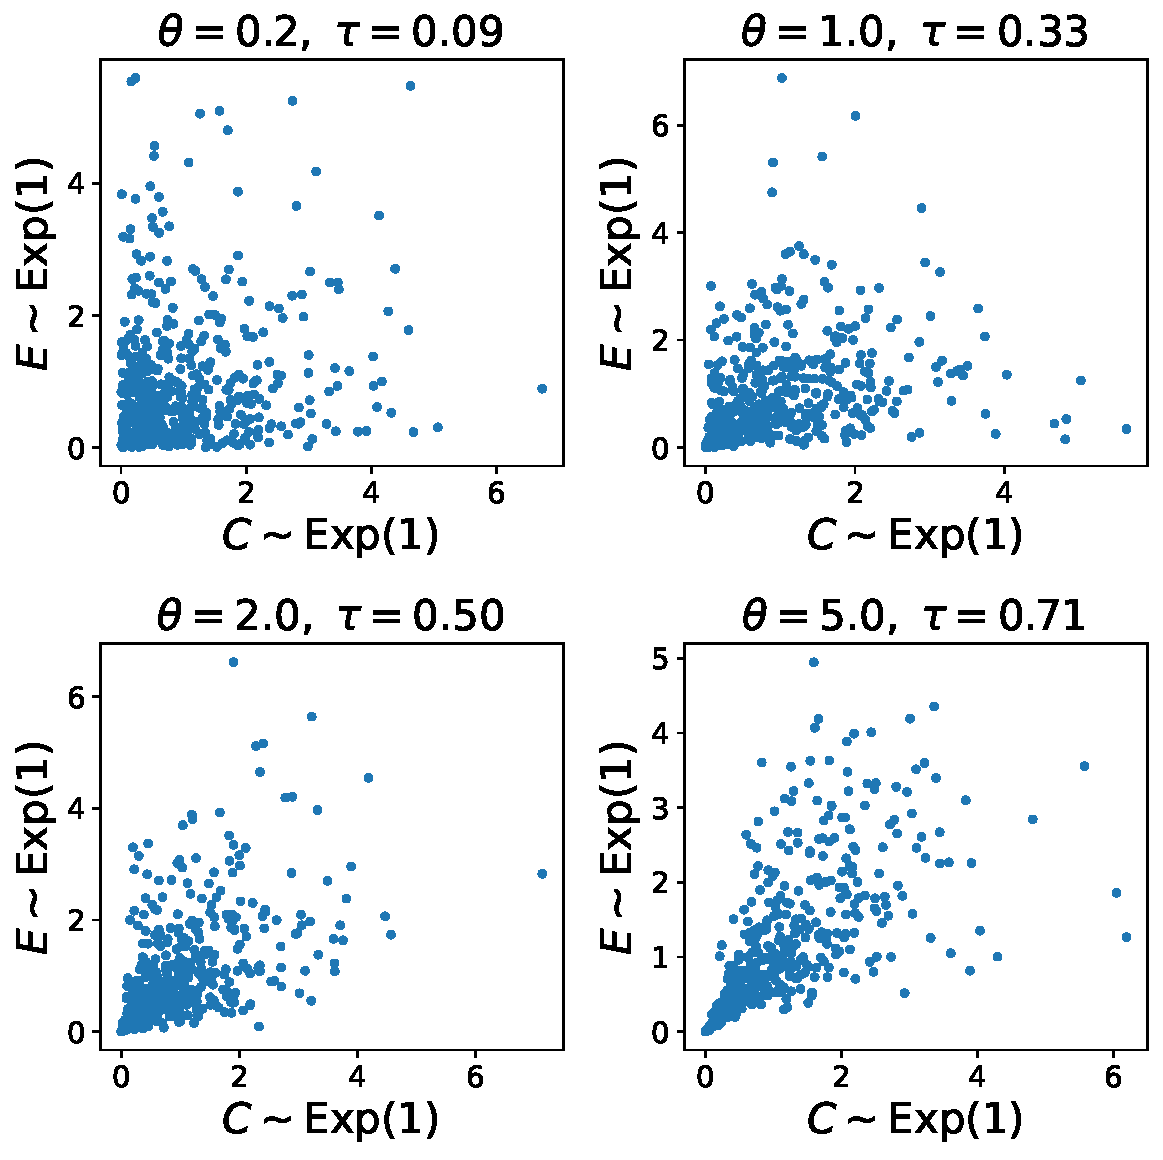
\includegraphics[width=\linewidth]{clayton_copula.pdf}
    \figsource{Figure from Lillelund et al.~\cite{lillelund_overcoming_2026}. Clayton copula on the CDFs (its original definition); our method applies it to $S_E$ and $S_C$.}
  \end{column}
\end{columns}
\end{frame}

\begin{frame}{Margin time of a censored patient}
\begin{columns}[c]
  \begin{column}{0.46\textwidth}
    \small
    A patient censored at $c$: when would the event have happened?
    \vspace{0.3em}

    \textbf{Margin time} \cite{haider2020effective} -- the expected event time, given survival past $c$:
    \[
      e^{\text{margin}} = c + \frac{\int_{c}^{\infty} \hat S(t)\, \d t}{\hat S(c)}
    \]
    \vspace{-0.4em}
    \begin{itemize}
      \item With Kaplan--Meier: $\approx 9.9$ -- far too late.
      \item With a copula-based estimate \cite{Zheng1995,Rivest2001}: $\approx 6.5$ (truth 6.6).
    \end{itemize}
  \end{column}
  \begin{column}{0.52\textwidth}
    \centering
    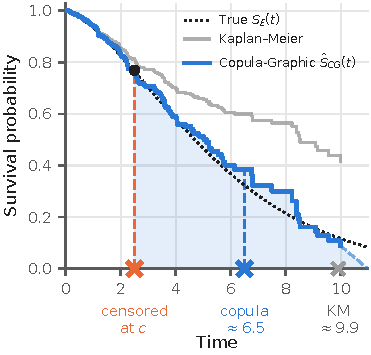
\includegraphics[width=\linewidth]{plot_margin_time_cg.pdf}
    \figsource{Simulated data, Clayton copula with $\tau = 0.5$.}
  \end{column}
\end{columns}
\end{frame}

\begin{frame}{The dependent Brier score (IBS-Dep)}
Replace each censored time by its copula-based margin time, and drop IPCW:
\[
  \text{BS}_{\text{Dep}}(t) = \frac{1}{\sum_i w_i} \sum_{i=1}^{N} w_i
  \Big(\mathbbm{1}\big[\tilde e_i > t\big] - \hat S(t \mid \bm{x}_i)\Big)^2
\]
\[
  \tilde e_i =
  \begin{cases}
    e_i & \delta_i = 1 \\
    e^{\text{margin}}(\hat S_{\text{CG}}, c_i) & \delta_i = 0
  \end{cases}
  \qquad
  \text{IBS}_{\text{Dep}} = \frac{1}{t_{\max}} \int_0^{t_{\max}} \text{BS}_{\text{Dep}}(\tau)\, \d\tau
\]
\vspace{0.2em}
\begin{columns}[T]
  \begin{column}{0.48\textwidth}
    \small
    \textbf{Uncertainty weighting (UW):}\\ $w_i = 1 - \hat S_{\text{CG}}(c_i)$ for censored patients -- early censoring tells us less.
  \end{column}
  \begin{column}{0.48\textwidth}
    \small
    \textbf{Guarantees:} margin time is consistent and asymptotically normal under the assumed copula.
  \end{column}
\end{columns}
\takeaway{Needs a copula family and parameter -- but no model of how censoring depends on the covariates.}
\end{frame}

\begin{frame}{Synthetic data: IBS-Dep stays accurate}
\small Simulated Weibull data, true copula known; error vs.\ the oracle IBS.
\vspace{0.3em}

\begin{columns}[T]
  \begin{column}{0.49\textwidth}
    \centering
    \footnotesize Increasing dependence (censoring 50\%)\\[0.2em]
    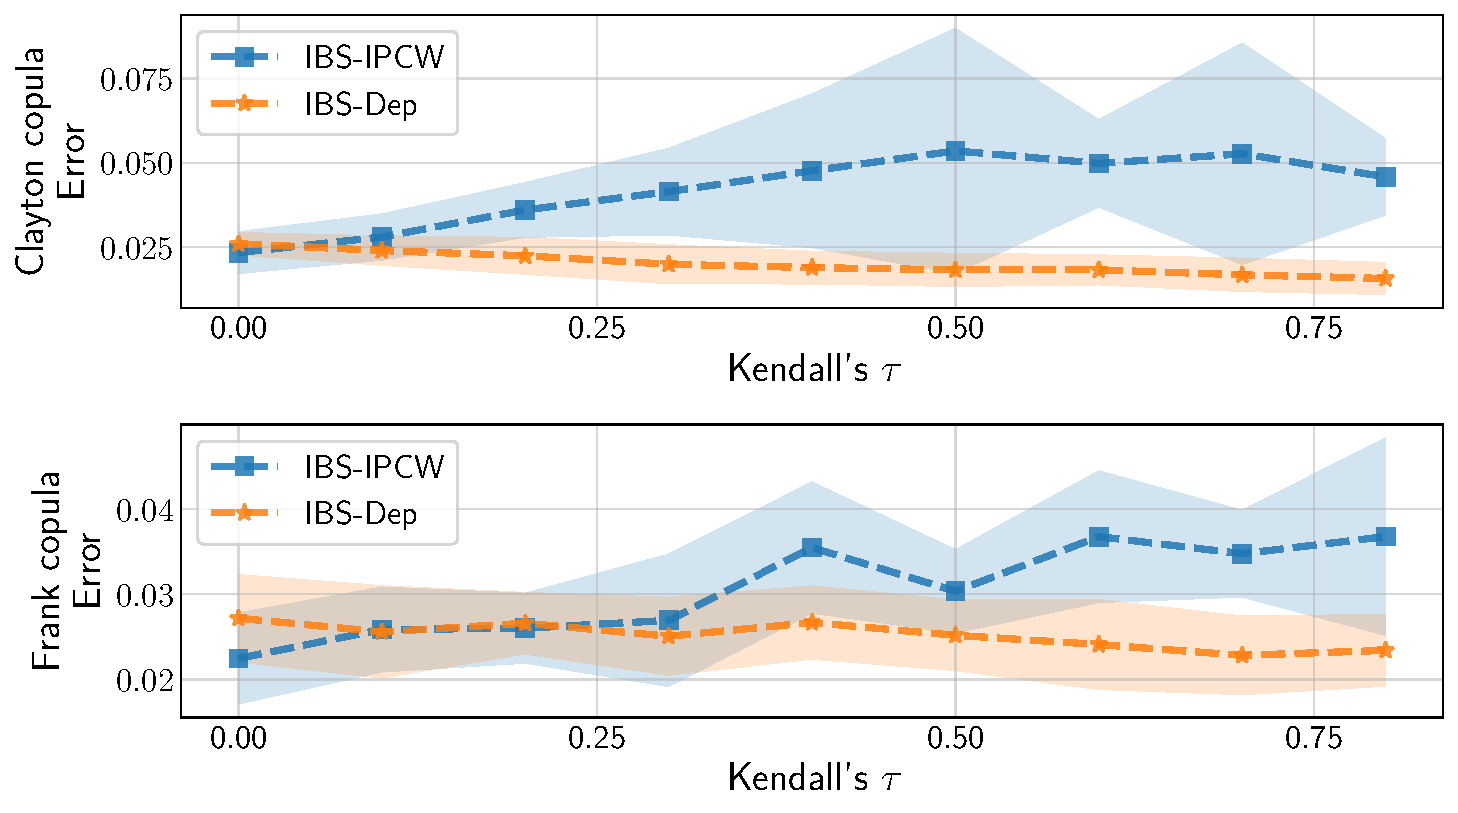
\includegraphics[width=\linewidth]{synthetic_correct_copula.pdf}
  \end{column}
  \begin{column}{0.49\textwidth}
    \centering
    \footnotesize Increasing censoring ($\tau = 0.5$)\\[0.2em]
    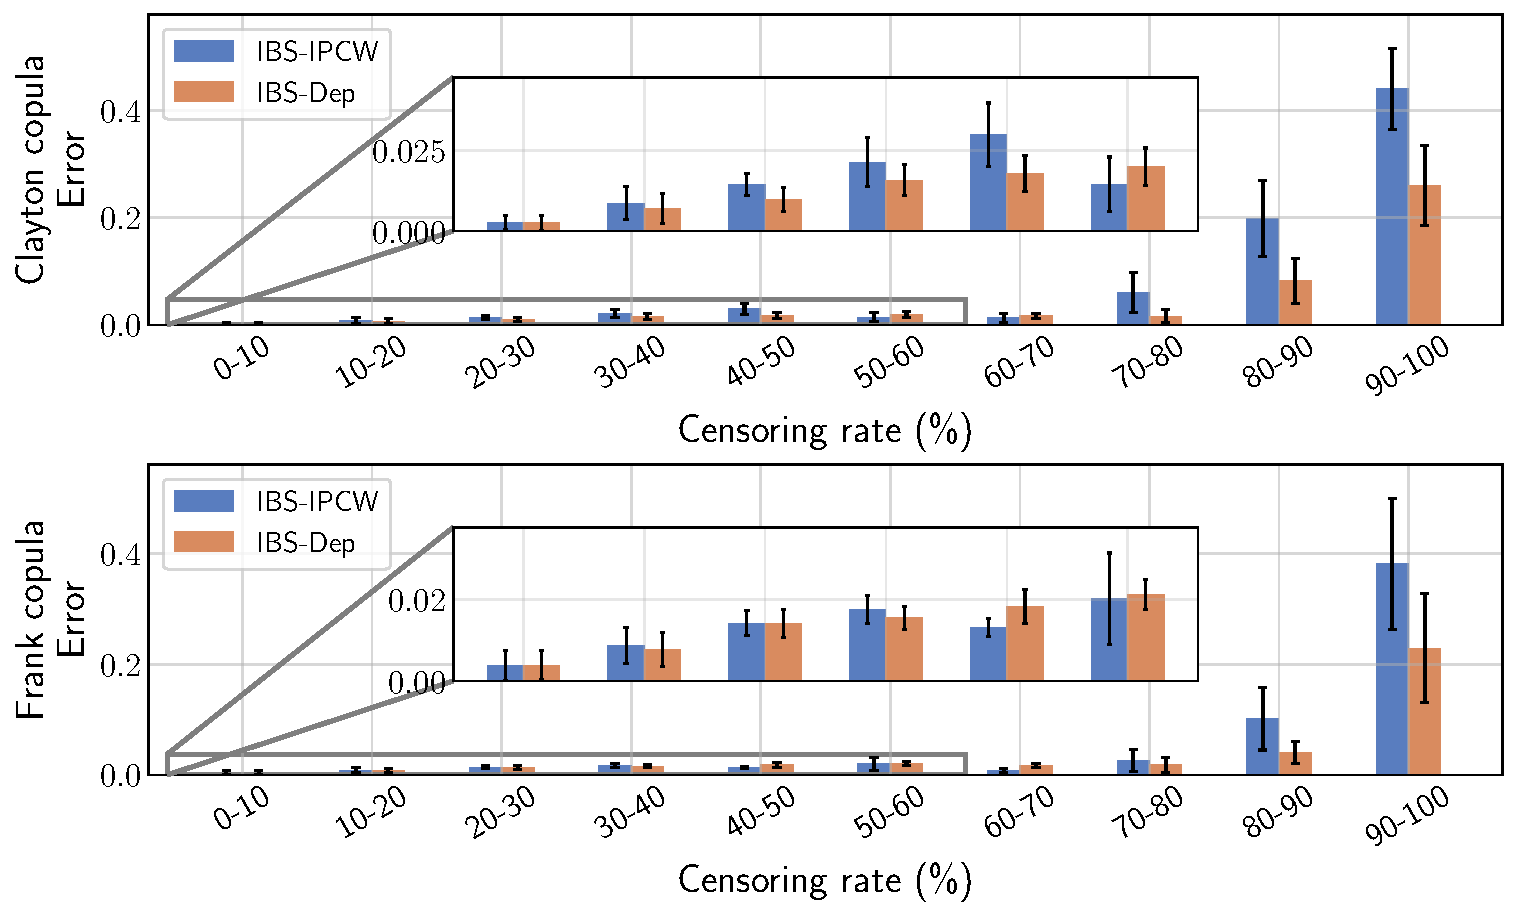
\includegraphics[width=\linewidth]{synthetic_censoring.pdf}
  \end{column}
\end{columns}
\figsource{Figures from Lillelund et al.~\cite{lillelund_overcoming_2026}}
\takeaway{IPCW error grows with dependence, and fast above $\sim$80\% censoring; IBS-Dep stays stable.}
\end{frame}

\begin{frame}{Less error, but no better at ranking}
\small 12 real datasets with resampled outcomes (true times known), dependence induced by dropping features. Left: error reduction vs.\ IPCW (KM). Right: how often a metric finds $\ge 2$ of the 3 best models.
\vspace{0.2em}

\centering
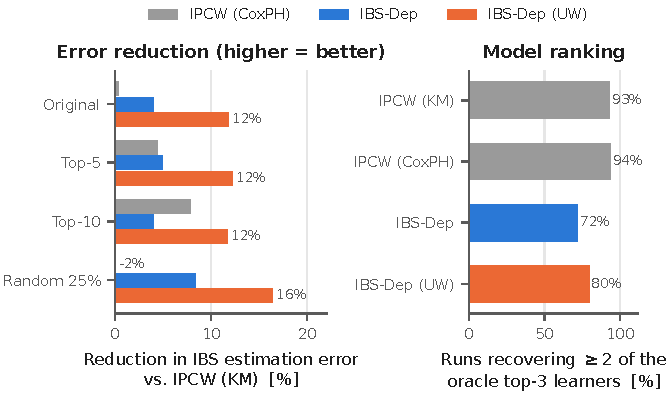
\includegraphics[width=0.8\linewidth]{plot_copula_results.pdf}
\figsource{Data from Lillelund et al.~\cite{lillelund_overcoming_2026}, averaged over 12 datasets.}
\end{frame}
